%! TEX root = thesis.tex

\chapter{Semiclassical physics}

\section{Multicomponent wave equations}

\subsection{A multicomponent eigenvalue problem}

In this section we will apply the results that we derived previously to a multicomponent problem whose solution is known exactly.
Consider the following multicomponent eigenvalue problem%
\footnote{These equations are slightly modified versions of the channel equations considered by~\citet{yabana1986}.}
%
\begin{equation}
  \begin{bmatrix}
    \left(\hat{a}^{\dagger}\hat{a} + \frac{1}{2}\right)\epsilon + \Delta & \mu\hat{a}^{\dagger}\\
    \mu\hat{a} & \left(a^{\dagger}\hat{a} + \frac{1}{2}\right)\epsilon - \Delta
  \end{bmatrix}
  \begin{bmatrix}
    \psi_{+}\\
    \psi_{-}
  \end{bmatrix}
  =
  E
  \begin{bmatrix}
    \psi_{+}\\
    \psi_{-}
  \end{bmatrix}.
\end{equation}
%
Above, $\Delta$ is a positive constant and the operators
%
\begin{equation}
\hat{a}^{\dagger} = \frac{x - i\hat{k}}{\sqrt{2\epsilon}}
  \quad\text{and}\quad
\hat{a} = \frac{x + i\hat{k}}{\sqrt{2\epsilon}},
\end{equation}
%
are the usual raising and lowering operators from quantum mechanics.%
\footnote{Here the parameter $\epsilon$ plays the role of the Planck's constant and we have set the mass and oscillator frequency to unity.}
Without the off diagonal terms, these equations reduce to two uncoupled simple harmonic oscillators, in which case the energies would be given by $E_{n}^{\pm} = (n + \frac{1}{2})\epsilon \pm \Delta$ for $n \in \mathbb{N}_{0}$.
To solve the eigenvalue problem in the presence of off-diagonal term, we expand the solution in terms of the eigenstates of the simple harmonic oscillator
%
\begin{equation}
  \psi_{+} = \sum_{n= 0}^{\infty} a_{n}\phi_{n}
  \quad\text{and}\quad
  \psi_{-} = \sum_{n = 0}^{\infty} b_{n}\phi_{n}.
\end{equation}
%
Putting the above equation in Eq.~XXX, we arrive at
%
\begin{equation}
   \begin{aligned}
     \sum_{n = 0}^{\infty} \left\{\left[\left(n +  \tfrac{3}{2}\right)\epsilon + \Delta - E\right]a_{n + 1} + \sqrt{n + 1}b_{n}\right\}\phi_{n+1}  + a_{0}\left(\tfrac{1}{2}\epsilon + \Delta - E\right)\phi_{0}&= 0\\
     \sum_{n = 0}^{\infty} \left\{\sqrt{n + 1}a_{n+1} + \left[\left(n +  \tfrac{1}{2}\right)\epsilon - \Delta - E\right]b_{n}\right\}\phi_{n} &= 0.
   \end{aligned}
\end{equation}
%
Since the $\phi_{n}$ are independent functions, their coefficients in the above equations should independently vanish, which leads us to the quantization condition.
Clearly, the lowest energy is $E = \tfrac{1}{2}\epsilon + \Delta$ and the associated eigenstate is $\psi = (0, \phi_{0})$.
%
\begin{equation}
  \begin{bmatrix}
    \left(n + \tfrac{1}{2}\right)\epsilon - \Delta - E & \sqrt{n + 1}\\
    \sqrt{n + 1} & \left(n + \tfrac{3}{2}\right) + \Delta - E
  \end{bmatrix}
  \begin{bmatrix}
    a_{n}\\
    b_{n + 1}
  \end{bmatrix}
  = 0.
\end{equation}
%



\begin{figure}
  \begin{center}
    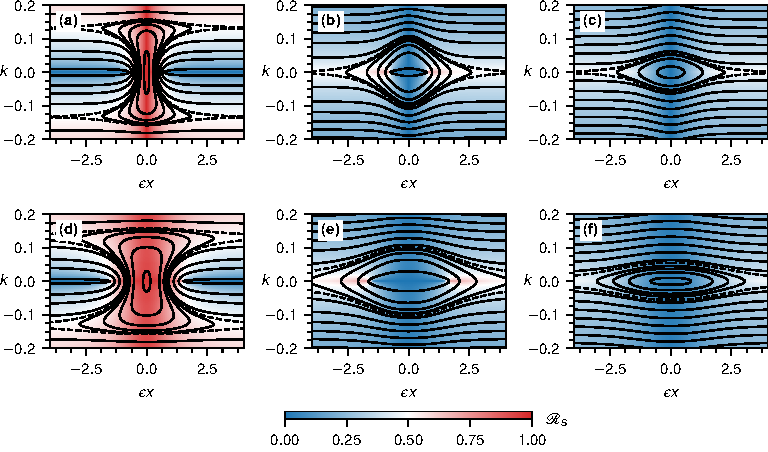
\includegraphics{shell_rays.pdf}
  \end{center}
\end{figure}

